%==============================================================================
\chapter{Introduction}\label{cha:chapter1}
%==============================================================================
%
%
%
\begin{remark}{Outline}
    In this chapter, we...
\end{remark}


%
%
%
\section{Physiology of the heart}
During each heartbeat, the chambers of the heart are activated by an electrical impulse that propagates across the entire tissue. The activation wave is initiated by a group of pacemaking cells, making up the \textit{sinoatrial node} and located in the right atria, and spreads throughout the ventricles via a specialised conduction system called \textit{His-Purkinje system}. The arrival of the activation wave at each cardiac cell or \textit{myocyte} causes a depolarisation of the cell membrane that initiates an \textit{action potential} (\acs{AP}). The electrical signal gives rise to a \textit{calcium transient} that activates the tension generating proteins inside the cell through a process called \textit{excitation-contraction} (\acs{EC}) coupling, causing concerted myocardial contraction and relaxation. \todo{missing picture of a full heart}


%
%
%
\subsection{Cardiac electrophysiology}\label{sec:cardiacelecphys}
The surface membrane of a cardiac cell is called \textit{sarcolemma}. On either side of the sarcolemma, the intracellular and the extracellular environments consist of ionic solutions. For cardiac electrophysiology the major ion species are sodium (\acs{Na}), potassium (\acs{K}), chloride (\acs{Cl}) and calcium (\acs{Ca}). An important property of the sarcolemma is its ability to maintain concentration gradients, such that each ion species is unevenly distributed between the intracellular and extracellular space, resulting in concentration gradients across the membrane. As ions are charged particles, their uneven distribution across the sarcolemma also creates an electrical gradient. The resulting electrochemical gradient drives the movement of ions across the cell membrane.

% \begin{figure}
%     \centering
%     \includegraphics{heart}
%     \caption{A picture of the heart and its conduction system}
%     \label{fig:my_label}
% \end{figure}

\vspace{0.2cm}
Another crucial property of the sarcolemma is its capacity to respond to electrical stimulation through the brief opening and closing of highly specific ion channels and electrogenic transporters to produce changes in its transmembrane potential. With each heartbeat, the cell membrane is depolarised and an AP is initiated as a result of a complex interplay of multiple ion channels and transporters in the myocardium. A typical AP consists of five phases, each one associated with the opening of specific sarcolemma ion channels. The main ionic events at each AP phase can be summarised as follows.

\begin{description}
	\item[\textsc{Phase $0$.}] The initial depolarisation is due to opening of voltage-gated fast $\Na$ channels ($I_{Na}$) when the transmembrane voltage reaches the activation threshold of the channel between $\SI{-70}{}$ and $\SI{-60}{\milli\volt}$. Positive charged $\Na$ current flows rapidly into the cell due to the large $\Na$ concentration gradient and the negative transmembrane potential, leading to further depolarisation.
	\item[\textsc{Phase $1$.}] The early repolarisation of the AP is primarily caused by the rapidly activating and inactivating transient outward $\K$ current ($I_{to}$).
	\item[\textsc{Phase $2$.}] A plateau phase following the previous described initial repolarisation, which results from a prolonged influx of $\Ca$ ions, as the voltage-gated L-type $\Ca$ channels ($I_{CaL}$) open upon depolarisation. This flow of $\Ca$ ions plays a crucial role in cardiac EC coupling, as it initiates a series of intracellular events that ultimately lead to myocardial contraction. Another current that contributes to the plateau phase is the net inward current through the $\Na$/$\Ca$ exchanger in $\Ca$ extrusion mode.
	\item[\textsc{Phase $3$.}] The outward flow of $\K$ ions is the major factor causing repolarisation that determines the duration of the AP. The large number of $\K$ channels can be divided into two molecular families: the voltage-gated channels and the inward rectifier channels. The voltage-gated outward $\K$ channels are the rapidly ($I_{Kr}$) and slowly ($I_{Ks}$) activating delayed rectifiers, and are responsible for repolarisation, fully activated at around $\SI{-10}{\milli\volt}$ and deactivated by full repolarisation. The inward rectifier $\K$ channels, such as the time-independent $\K$ current $I_{K1}$, help regulating the resting membrane potential and contribute to late Phase $3$ repolarisation.
	\item[\textsc{Phase $4$.}] $I_{K1}$ closes upon depolarisation and reopens during repolarisation to help terminate the AP and reset the membrane potential to the resting state, which for non-pacemaker cardiac cells such as the ventricular myocytes is around $\SI{-90}{mV}$.
\end{description}

\begin{figure}[!ht]
    \myfloatalign
    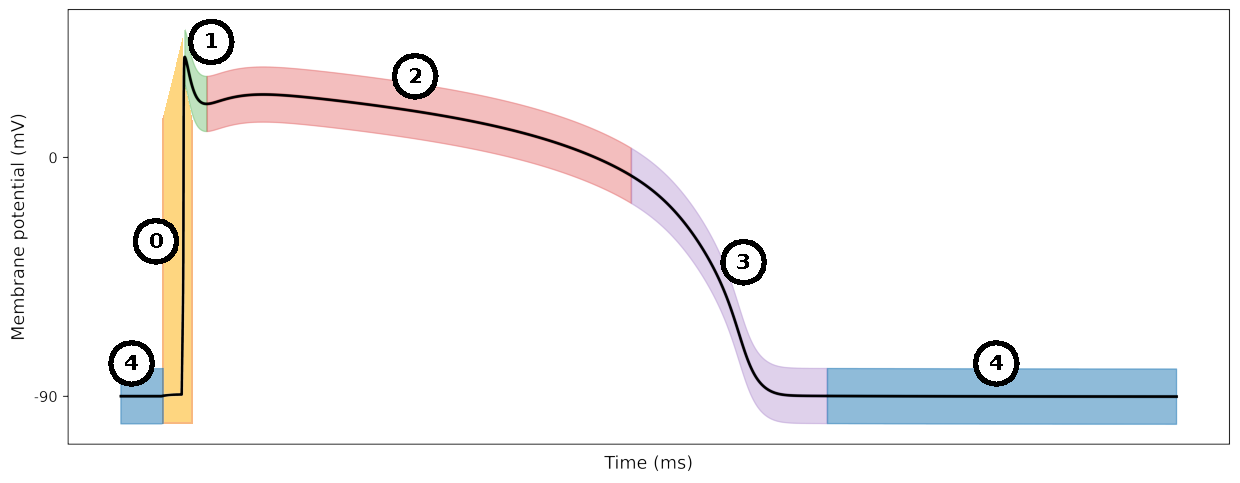
\includegraphics[width=\textwidth]{figures/chapter01/AP_phases.pdf}
    \caption{The five phases of an action potential in left ventricular myocytes.}
    \label{fig:my_label}
\end{figure}

\vspace{0.2cm}
The ionic uneven displacement across the sarcolemma constituting the resting membrane potential and required for the movement of ions during an AP is actively maintained by a number of membrane exchangers and pumps and is the result of a perfect balance between ions having flowed into and out the cell at each beat. The $\Na$/$\K$ \textit{ATPase} (\acs{NAK}) is a key transporter and uses energy (in the form of adenosine triphosphate (\acs{ATP})) to establish a low intracellular $\Na$ concentration and a high intracellular $\K$ concentration by moving $3$ $\Na$ ions out and $2$ $\K$ ions into the cell by hydrolisation of $1$ ATP molecule. This transport is electrogenic, as it results in the extrusion of $1$ net charge per cycle. The $\Na$/$\Ca$ \textit{exchanger} (\acs{NCX}) is another important transporter that maintains the $\Ca$ concentration gradient. This exchanger is a reversible counter-transport system that, when in forward ($\Ca$ extrusion) mode, uses the energy provided by the inward flux of $\Na$ ions down their electrochemical gradient to extrude $\Ca$ ions with a generally accepted stoichiometry of $3\colon 1$, thus moving one net charge into the cell per cardiac cycle.

\vspace{0.2cm}
Every ventricular myocyte is in general not excitable (\textit{refractory}) during Phase $0$, $1$, $2$ until half way through Phase $3$. This means that the cell cannot produce another AP (\textit{absolute refractory period}). However, after this moment and until the end of Phase $3$ during repolarisation (\textit{relative refractory period}), the cell can potentially evoke a new AP although needing a larger-than-normal excitatory stimulus. This is due to most of the $\Na$ channels still being inactivated and to a $\K$ ions leak which makes the membrane potential being more negative than the resting configuration (\textit{hyperpolarisation}). Myocytes' non-excitability has two major implications. The first one concerns the spread of excitation through the heart which is brought about by local electrical currents that act ahead of the action potential. In the depolarised, active region the membrane interior is positively charged, while the resting region ahead is negatively charged. The two internal regions are connected through a conductive pathway called \textit{gap junction}, and positive charge can therefore flow to the resting membrane region, depolarising it. Conversely, in the extracellular space positive charge flows from the resting membrane region to the active region. When in the resting region the membrane potential reaches the threshold for voltage-gated $\Na$ channels opening (Phase $0$), the rear, previously active region is still in its refractory period, therefore the excitation can only proceed unidirectionally. The second major implication concerns myocyte contraction. As we shall see in Section~\ref{sec:cardiaccellcontr}, cell contraction takes place in response to an increase in intracellular $\Ca$ concentration (\acs{Cai}). The peak mechanical event (maximal contraction) is achieved after the peak chemical event (maximal $\Cai$) which is achieved after the peak electrical event (maximal membrane potential). More specifically, peak tension is reached during the AP absolute refractory period while the myocyte relaxes during the AP relative refractory period, so that tension development is completed before the myocyte becomes excitable again. The contractile behaviour of the heart is thus restricted to repeated single \textit{twitches}, preventing life threatening sustained myocardial contractions.

\begin{figure}[!ht]
    \myfloatalign
    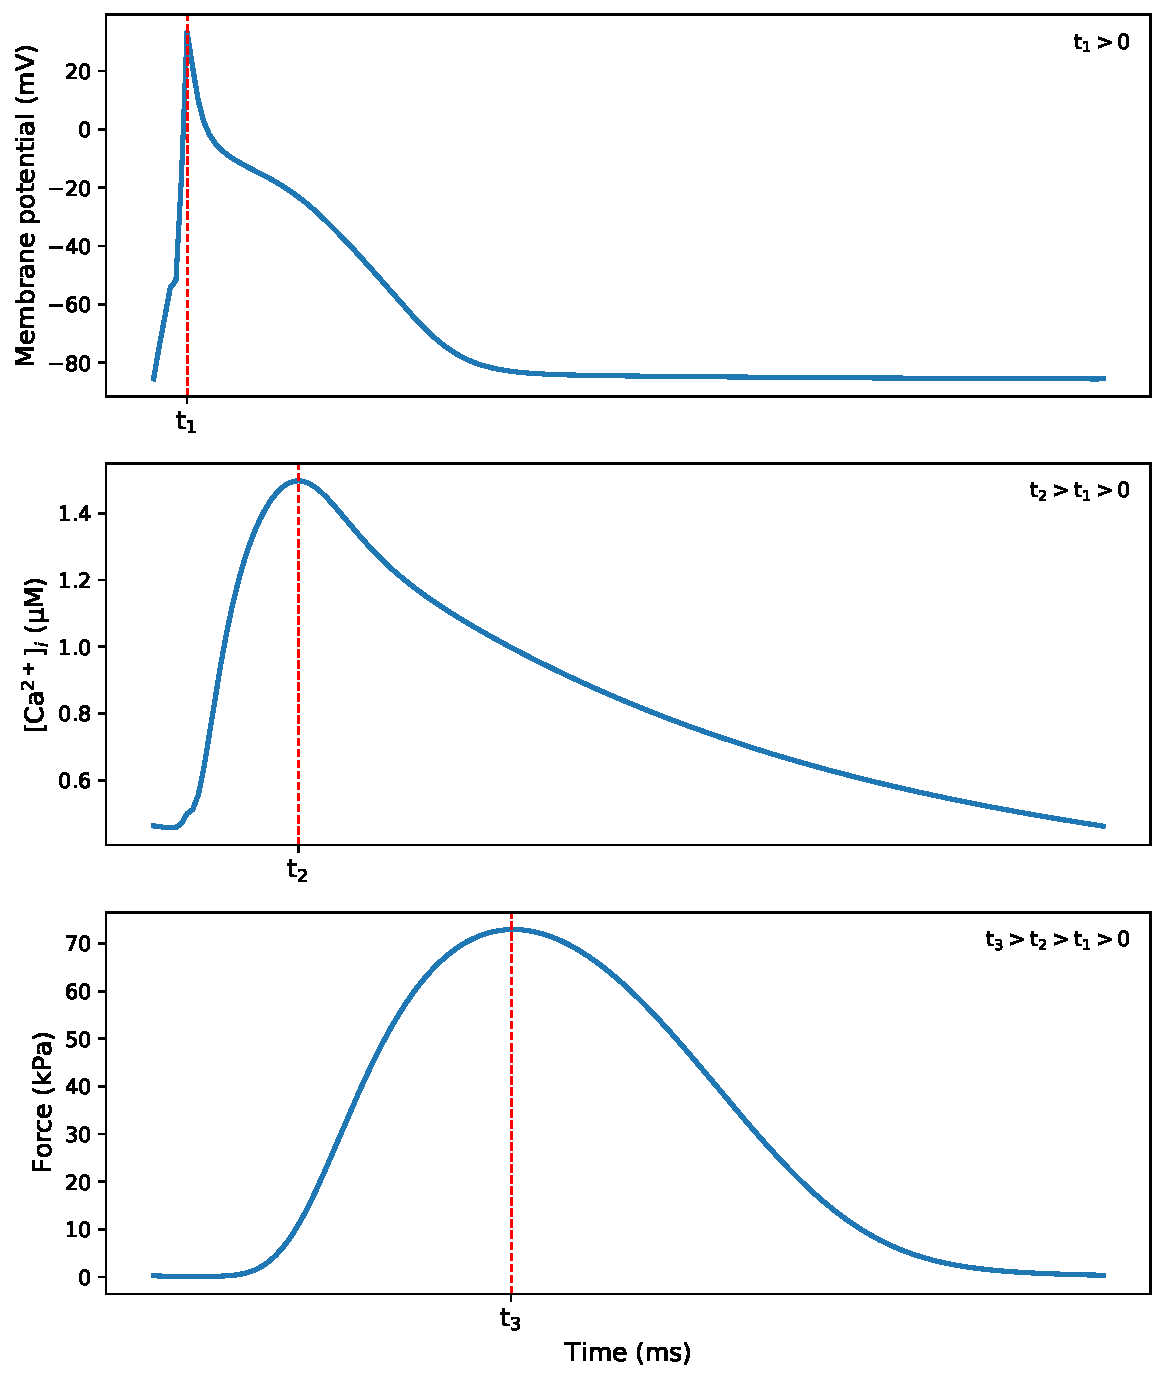
\includegraphics[width=0.66\textwidth]{figures/chapter01/three_peaks.pdf}
    \caption{Example action potential, calcium transient and twitch transient in the rat left ventricular myocyte. From the top to bottom, the three curves are clearly peaking at three successive time points $t_1,\,t_2,\,t_3$.}
    \label{fig:my_label1}
\end{figure}

% [\textbf{TODO}: differences across species]
% Ion currents dynamics may vary a lot across animal species, and this results in different AP shapes, as in the case of humans compared to mice and rats. In Figure~\ref{fig:apcomp}, human and mouse APs are shown. Although most ion channels are conserved across species, there are significant differences in the potassium currents involved in repolarization between human and mouse ventricular myocytes \cite{nerbonne2004}. Specifically, although the upstroke is similar in both species, the repolarization phase shows clear differences. In humans, the upstroke is followed by transient repolarization and a plateau phase, whereas in mice no plateau is visible and repolarization is rapid.

% \begin{figure}
%     \centering
%     \includegraphics[scale=0.4]{figures/ap_human_mouse_comp.png}
%     \caption{Ventricular action potential and currents for human (left) and mouse (right). Credit: \cite{nerbonne2004}}
%     \label{fig:apcomp}
% \end{figure}


%
%
%
\subsection{Cardiac cellular contraction}\label{sec:cardiaccellcontr}
The basic contractile unit of each myocyte is called \textit{sarcomere} and is mainly composed of filamentous proteins (\textit{myofilaments}) between thin partitions called \textit{Z lines}. The two principal interdigitating myofilaments are composed respectively of \textit{myosin} protein (\textit{thick filament}) and of \textit{actin} protein (\textit{thin filament}). The thin filament consists of two actin strings arranged as a two-stranded helix, which groove contains two regulatory proteins: \textit{tropomyosin} (\acs{Tn}) and \textit{troponin} (\acs{Tm}). The sarcomere also contains spring-like filaments of \textit{titin}, connecting Z lines. They ensure that myosin filaments stay aligned and they confer elasticity to the heart wall along with the extracellular \textit{collagen}. \todo{missing picture of the thin and thick filaments}

\vspace{0.2cm}
Heart contraction is the result of sarcomere shortening, which is the result of thin filaments sliding into the thick filaments space. Myofilaments movement past each other is possible because of a repeated making, rotation and breaking of biochemical bonds between the thin and the thick filaments called \textit{crossbrigdes}. Crossbridges are simply myosin heads protruding from the side of the thick filament when they are attached to the thin filament. Their movement after being anchored and consequent detachment in turns shortens the sarcomere. Each single head represents an independent generator of force: the force generated within the entire sarcomere is therefore the cumulative contribution of many myosin heads.

\vspace{0.2cm}
It is clear that the myofilaments effectively constitute the contractile machinery within the sarcomere. However, these can only initiate contraction in a $\Ca$-dependent manner. At rest when $\Cai$ is low, the thin filament regulatory Tn-Tm complex in fact blocks the myosin binding sites on actin, thereby sterically preventing crossbridges formation and tension generation. As $\Cai$ rises, $\Ca$ ions bind to the calcium-binding subunit of Tn, namely \textit{troponin C} (\acs{TnC}), and enable the movement of the Tn-Tm complex to expose the binding sites and allow acto-myosin interaction.


%
%
%
\subsubsection{The role of calcium}
Calcium plays a key role for the cardiac cell to contract. The variation of $\Ca$ levels observed inside the cell during each cardiac cycle is referred to as \textit{calcium transient} or \textit{calcium signal}. To understand the $\Ca$ dynamics that makes the common $\Cai$ transient shape, we need to introduce other important both structural and functional myocyte components.

\vspace{0.2cm}
Cardiac myocytes have a long cylindrical shape. The sarcolemma encapsulating the cell invagenates and forms an extensive tubular network called \textit{transverse} (\acs{T}) \textit{tubules} which allows the AP to penetrate rapidly to the interior of the cell. Next to the T-tubules inside the cell lies the terminal cisternae of the \textit{sarco(endo)plasmic reticulum} (\acs{SR}), forming a closely coupled structure called \textit{dyad}. The SR contains a store of $\Ca$ ions, which are partially released into the \textit{sarcoplasm} (another name for the cytoplasm within the sarcolemma) when the cell is excited. As the AP travels along the sarcolemma and along the T-tubules, $\Ca$ enters the cell through the L-type $\Ca$ channels. $\Ca$ then binds to and activates the \textit{ryanodine receptors} (\acs{RyR}s), which are $\Ca$ release channels located on the SR, triggering further release of a much greater number of $\Ca$ ions from the SR. This process is termed \textit{calcium-induced calcium release}. $\Ca$ diffuses from the dyadic space into the cytosol, and then diffuses to the sarcomeric proteins and binds to TnC leading to contraction.

\vspace{0.2cm}
Relaxation occurs as $\Ca$ is removed from the cytosol, lowering $\Cai$ such that $\Ca$ dissociates from TnC. $\Ca$ removal is achieved either via $\Ca$ extrusion from the cell or $\Ca$ uptake into intracellular $\Ca$ stores. Two mechanisms are known to be responsible for the extrusion of $\Ca$ from myocytes: NCX and the \textit{plasma membrane} $\Ca$ \textit{ATPase} (\acs{PMCA}). The majority of the $\Ca$ entering the cytosol during a $\Cai$ transient is taken up back into the SR via the \textit{sarcoplasmic} $\Ca$ \textit{ATPase} (\acs{SERCA}), with $2$ $\Ca$ ions transported into the SR for every $1$ ATP molecule consumed.

\vspace{0.2cm}
We have seen that $\Ca$ homeostasis is maintained via a careful balancing of $\Ca$ fluxes through different transporters and channels.
When the balance of inward and outward $\Ca$ (but also other ions) currents is upset, the homeostasis is disrupted: this phenomenon is known to be at the base of many life threatening cardiovascular diseases.


%
%
%
\subsection{Cardiac physiologic anatomy and hemodynamics}
The heart is composed of two muscular pumps, the right and left ventricles (\acs{RV}, \acs{LV}), each one filled from a contractile reservoir, respectively the right and left atria (\acs{RA}, \acs{LA}). The \textit{cardiac cycle} consists of a period of relaxation called \textit{diastole}, during which the heart fills with blood, followed by a period of contraction called \textit{systole}.

\vspace{0.2cm}
Atria and ventricles are separated by fibrous tissue surrounding two openings called \textit{atrioventricular valves}. Venous blood (\textit{superior} and \textit{inferior} \textit{venae cavae} and \textit{coronary sinus} for RA, four \textit{pulmonary veins} for LA) normally flows to the atria and then up to $\SI{80}{\percent}$ goes directly into the ventricles. Atrial contraction serves as primer pump to additionally fill the ventricles with the remaining $\SI{20}{\percent}$, although this percentage increases with age. The volume of blood in a ventricle at the end of its \textit{filling} is called \textit{end-diastolic volume} (\acs{EDV}), while the corresponding same chamber pressure is called \textit{end-diastolic pressure} (\acs{EDP}). Atrial systole is followed by ventricular systole. This is accompanied by a sharp ventricular pressure rise above the atrial pressure which makes the atrioventricular valves close by reversed pressure gradient, preventing retrograde blood flow. However, as the developed pressure is not yet sufficient to push the \textit{aortic valve} and the \textit{pulmonary valve} (respectively connecting the LV, RV with the \textit{systemic} and \textit{pulmonary} circulations) open, ventricles contraction initially occurs with no emptying. Cardiac muscle tension is thus increasing but little or no shortening of the muscle fibres is occurring, producing an \textit{isovolumetric contraction} (\acs{IVC}) with further pressure increase. When the ventricular pressure exceeds the arterial pressure, this opens the aortic and pulmonary valves and we have \textit{ejection} of blood. The ejected blood volume also called \textit{stroke volume} (\acs{SV}) is only about two-thirds of the available EDV of blood: a residual blood volume, namely the \textit{end-systolic volume} (\acs{ESV}), is kept as a reserve to be drawn on to raise the stroke volume in specific circumstances (e.g. during exercise). The proportion of ejected blood, i.e. SV divided by EDV, takes the name of \textit{ejection fraction} (\acs{EF}). The ejection rate is initially rapid and then progressively slows down. Since the rate at which the aortic blood is draining away into the peripheral circulation now exceeds ventricular ejection, also ventricular pressure begins to fall until reaching the \textit{end-systolic pressure} (\acs{ESP}) when the outflow valves close. At this point, both the ventricles become close chambers again, and a rapid pressure fall occurs driven by the elastic recoil of the deformed, relaxing myocardium. This process takes place at constant blood volumes and is called \textit{isovolumetric relaxation} (\acs{IVR}). When the intraventricular pressures decrease back to their low diastolic levels, the atrioventricular valves open and blood floods in from the atria (which have themselves been filling up during ventricular systole) and the next cardiac cycle begins.

\vspace{0.2cm}
To summarise, isovolumetric contraction, ejection, isovolumetric relaxation and filling are the $4$ main phases of the cardiac cycle (summarised in Figure).

\begin{figure}[!ht]
    \myfloatalign
    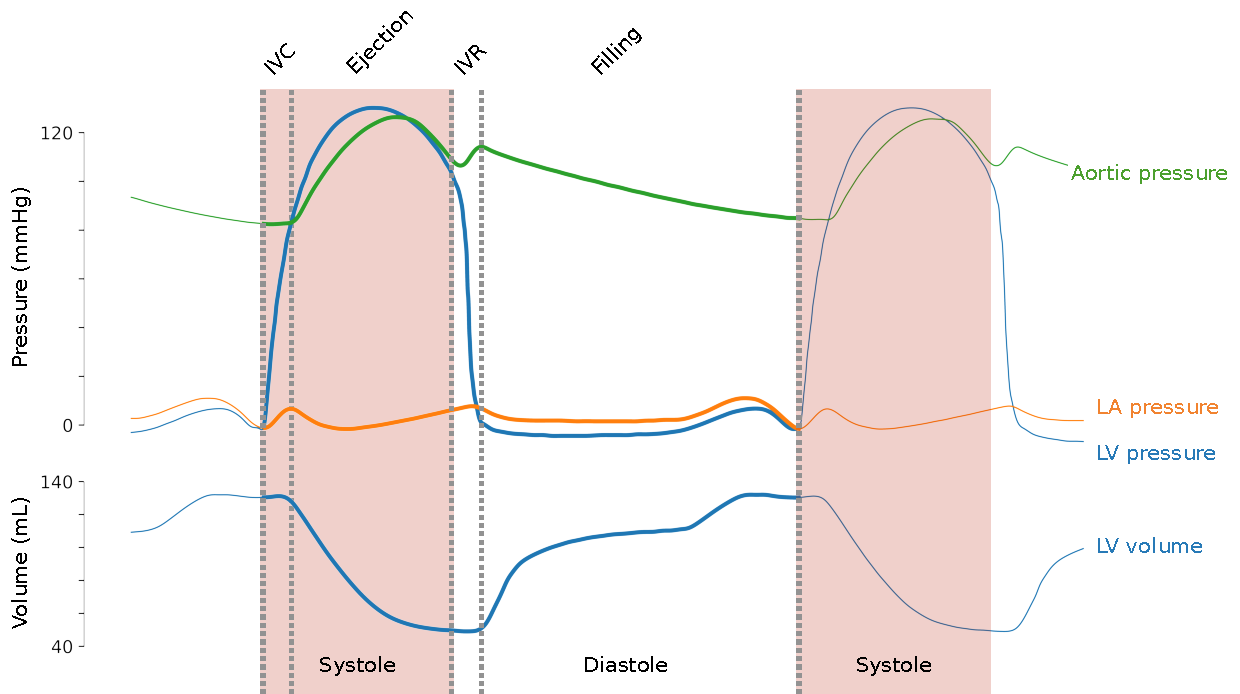
\includegraphics[width=\textwidth]{figures/chapter01/wiggers_diagram.pdf}
    \caption{Wiggers diagram representing the four main phases of the cardiac cycle in the left heart.}
    \label{fig:wiggersdiagram}
\end{figure}


%
%
%
\section{Mathematical modelling of the heart}
Biophysically detailed mathematical models have been developed to better understand cardiac physiology at each different scale of the system, from cell to the whole-organ levels, and to gain insight into the pathophysiology of complex cardiovascular diseases and help interpret clinical observations to improve patients treatment.


%
%
%
\subsection{Cell electrophysiology}
% Cardiac electrophysiology has been measured in the clinic for more than ten decades. These measurements have proved to be essential for patient diagnoses and monitoring. Computational models of cardiac electrophysiology have more recently been employed to interpret clinical data.
% \vspace{0.2cm}
In Section~\ref{sec:cardiacelecphys}, we have seen how ions uneven distribution across the interior and the exterior of the sarcolemma is essential for a correct AP generation. The equilibrium potential for a particular ion at which its electrochemical gradient is balanced can be expressed through the \textit{Nernst equation}:
%
\begin{equation}\label{eq:nernsteq}
    E_{\textrm{ion}}=\frac{\textrm{R}\textrm{T}}{\textrm{F}z}\,\ln{\frac{[\textrm{ion}]_{\textrm{ex}}}{[\textrm{ion}]_{\textrm{in}}}}
\end{equation}

\noindent
where

\vspace{0.2cm}
\begin{tabular}{ll}
    $\textrm{R}$  & gas constant \\
    $\textrm{T}$  & absolute temperature \\
    $\textrm{F}$  & Faraday's constant \\
    $z$           & ion valence \\
    $[\textrm{ion}]_{\textrm{in}}$  & ion intracellular concentration \\
    $[\textrm{ion}]_{\textrm{ex}}$  & ion extracellular concentration \\
\end{tabular}

\vspace{0.5cm}
Ionic cell models have been developed to represent the baseline physiology of both atrial, ventricular, and sinoatrial node myocytes [REFS]. Also, a variety of many other models have been built~\cite{Corrado:2020} by adapting these first, general one to specifically interpret clinical data from pathological phenotypes (e.g. gene mutation causing a specific ion channel malfunction). These many currently available models all share some traits and mostly differ in single ion channels kinetics representations.

\vspace{0.2cm}
The sarcolemma is commonly viewed as an electrical circuit (\textit{equivalent circuit model}), comprised of a capacitor in parallel with resistors that represent ionic currents. The total membrane current is given as the sum of the capacitive current and the ionic current:
%
\begin{equation}
I_m = C_m\,\der{V_m}{t} + \sum_{\textrm{ion}}I_\textrm{ion}
\end{equation}

\noindent
where

\vspace{0.2cm}
\begin{tabular}{ll}
    $I_m$            & total membrane current \\
    $I_\textrm{ion}$ & individual transmembrane ionic current with sign \\ & (negative, positive for inward, outward currents respectively) \\ 
    $C_m$            & capacitance of the cell membrane per unit area \\
    $V_m$            & transmembrane voltage
\end{tabular}

\vspace{0.5cm}
\noindent
and the generic transmembrane current $I_{\textrm{ion}}$ is described as:
%
\begin{equation}
    I_{\textrm{ion}} = g_{\textrm{ion}}\,(V_m-E_{\textrm{ion}})
\end{equation}

\noindent
where

\vspace{0.2cm}
\begin{tabular}{ll}
    $g_{\textrm{ion}}$ & average channel conductance \\
    $V_m$ & transmembrane voltage \\
    $E_\textrm{ion}$ & Nernst potential (equation~\eqref{eq:nernsteq}) of the considered ion species
\end{tabular}

\vspace{0.5cm}
Now, the current $I_{\textrm{ion}}$ is produced by the movement of individual ions across the membrane through an ion channel, which is made of pore-forming proteins that span the membrane lipid bi-layer. Ion channels are regulated by a \textit{gate} which allows ions to pass according to whether it is in its open or closed state. Changes in an ion channel conformation takes place in response to chemical or electrical signals, temperature, or mechanical force. Cardiac cells ion channels are mostly \textit{voltage-gated}, meaning that they change conformation with varying transmembrane voltage. Two approaches have been used to represent ionic channels kinetics: the first uses the Hodgkin-Huxley (\acs{HH}) formulation~\cite{Hodgkin:1952} while the second (a generalisation of the first) uses continuous-time Markov chain models (\acs{MM})~\cite{Fink:2009}.

\vspace{0.2cm}
In the HH characterisation of channels the conductance is given by the product of a maximal conductance term and one or more separate \textit{gating variables} that represent the probability of finding the channel open:
%
\begin{equation}
    g_{\textrm{ion}} = g_{\textrm{ion}}^{\textrm{max}}\times y_i\cdot\dots\cdot y_N
\end{equation}

\noindent
where each gating variable $y:=y_i$ can be formulated using the equation:
%
\begin{equation}
    \der{y}{t} = \frac{y_{\infty}-y}{\tau_y}
\end{equation}

\noindent
where

\vspace{0.5cm}
\begin{tabular}{ll}
$y_{\infty}$ & voltage-dependent steady-state function of the gate \\
$\tau_{y}$ & voltage-dependent time constant
\end{tabular}

\vspace{0.5cm}
\noindent
The gating variables described in the HH formulation do not represent specific kinetic states of the ion channel. Moreover, they are assumed to be independent.

\vspace{0.2cm}
To accurately describe the dependence of a given transition on the occupancy of different states for a given channel, MMs are used. In this case, a discrete number of states represent the possible configurations a channel has. Transitions from one state to the other can occur at different rates, and the rate zero is used by convention when no direct switching between two given states is possible. Gating variables will then simply represent the probability of finding the channel in the respective states (\textit{state variables}). An example of MM approach to model an ion channel which can be either in the open, closed or inactivated configuration includes $3$ state variables to represent the three possible configurations and $6$ transition rates. Variation of state $y_i$ is given as a function of the other state variables $y_j$ for $j\in\{1,2,3\}\setminus{\{i\}}$:
%
\begin{equation}
    \der{y_i}{t} = \sum_{\substack{j=1 \\ j\neq i}}^{3} (k_{ji}\,y_j-k_{ij}\,y_i)
\end{equation}

\noindent
being $k_{ji}\in\mathbb{R}$ the rate at which transition from state $y_j$ to state $y_i$ occurs.

\vspace{0.5cm}
It is worth mentioning that the two presented HH and MM modelling frameworks are not mutually exclusive but are instead very frequently used in combination to differently represent the many ion channels within the cell. According to how many channels are represented using MMs and with how many states, electrophysiological cell models can thus be of increasing complexity.

% \vspace{0.2cm}
% \cite{hinch2004, pandit2001, gattoni2016}. In this study, the rat ventricular electrophysiology and calcium dynamics are described by employing Gattoni et al. \cite{gattoni2016} model, fitted to consistent experimental data in both SHAM and AB rats at physiological frequency and temperature \cite{gattoni2017}.


%
%
%
\subsection{Cell contraction}\label{sec:mathcellcontr}
Cardiac contraction models are used to simulate active tension generation at the sarcomere level arising from the thin and thick filaments. These models development has proceeded over the years in parallel with key experimental discoveries about striated and cardiac muscle physiology~\cite{Niederer:2019}. We have gone from simple phenomenological models aiming to represent the average sarcomere dynamics to very complex, spatially detailed models trying to capture the explicit positions of individual molecules. However, in the view of incorporating these models within whole-organ computational frameworks, currently adopted sarcomere contraction models have achieved a balance between recapitulating the main mechanistic phenomena while still being represented by a few number of ordinary differential equations (\acs{ODE}s) to be computationally efficient to solve. Key mechanisms regulating sarcomere contraction it is desirable to capture include force dependence on sarcomere length (\textit{Frank-Starling mechanism}), myofilament cooperative activation by $\Ca$, acto-myosin cooperative interaction in crossbridges formation, force dependence on sarcomere length variation (velocity).

% Models have been developed with a wide spectrum of complexity, going from the will of capturing the explicit positions of individual molecules to simply aiming to represent the average sarcomere dynamics \cite{Niederer:2019}. Whole organ modelling relies on the latter models, due to their computational efficiency. An example of this kind of models is given by the rat heart contraction model developed by Land et al. \cite{land2012a}, based on the relevant two works of Niederer, Hunter $\&$ Smith \cite{niederer2006} and Rice, Wang $\&$ de Tombe \cite{rice2008}. This model simulates troponin C, tropomyosin and crossbrigde dynamics and predicts the tension generated by cardiac muscle in response to changes in $\Ca$, length and velocity. 

% %
% %
% %
% \vspace{0.5cm}
% \textbf{Modelling $\Ca$ dependence}

% \vspace{0.2cm}
% The Land et al. \cite{land2012a} equation for troponin binding captures the cooperativity experimentally observed in calcium binding to the second binding site on troponin C (TnC), and has a Hill curve as steady-state solution:

% \begin{equation}\label{eq:trpneq}
%     \frac{d\trpn}{dt} = k_{\trpn}\,\left[\left(\frac{\Cai}{\Caift}\right)^{n_{\trpn}}(1-\trpn)-\trpn\right]
% \end{equation}

% where $\trpn$ represents the fraction of occupied regulatory sites, $k_{\trpn}$ the unbinding rate and $n_{\trpn}$ the Hill coefficient. The process of calcium binding to TnC causes a conformational change in its associated tropomyiosin complex, unblocking the actin sites for myosin crossbridge cycling. In Land et al. work, differently from the previous work of Rice et al. \cite{rice2008}, the crossbridge cycle has been collapsed to a single state, yielding a model with only two states: (1) the crossbridge state $\xb$ in which the crossbridge is actively cycling, and (2) the non-permissive state $1-\xb$. As in equation~\ref{eq:trpneq}, also the expression for the transition between these two states has been chosen to give a Hill curve in the steady-state:

% \begin{equation}\label{eq:xbeq}
%     \dfrac{d\xb}{dt} = \kxb\,\left[\permtot\,(1-\xb)-\frac{1}{\permtot}\,\xb\right]
% \end{equation}

% where

% \begin{equation}
%     \permtot := \sqrt{ \left( \frac{\trpn}{\trpnf} \right) ^{\nxb} }
% \end{equation}

% and being $\kxb$ the unbinding rate and $\nxb$ the Hill coefficient.

% % \begin{figure}[H]
% %     \centering
% %     \includegraphics[width=0.6\textwidth]{figures/land_et_al.png}
% %     \caption{Framework of the cell contraction model and its interaction at tissue scale in Land et al. model \cite{land2012a}.}
% % \end{figure}

% %
% %
% %
% \vspace{0.5cm}
% \textbf{Length- and velocity-dependence}

% \vspace{0.2cm}
% For developing models of cardiac muscle, detailed data on the velocity-dependent response are often required. These data are fitted to the function proposed by Kawai et al. \cite{kawai1993}:

% \begin{equation}\label{eq:eqkawaii}
%     y(f) = H - \frac{B\,i\,f}{b+i\,f}+\frac{C\,i\,f}{c+i\,f}+\frac{D\,i\,f}{d+i\,f}
% \end{equation}

% In the Land et al. model \cite{land2012a}, length- and velocity-dependent processes were taken into account in the normalized generated force expression as follows:

% \begin{equation}\label{eq:normforce}
%     F_n = g(Q)\cdot h(\lambda)\cdot \xb
% \end{equation}

% where $g(Q)$ determines the velocity dependence and $h(\lambda)$ the change in maximum force, being $\lambda$ the extension ratio along the fibre direction. The increase in maximum force was based on filament overlap and modelled using the same approach adopted by Rice et al. \cite{rice2008}:

% \begin{align}
%     h'(\lambda) &= 1+\beta_0\,[\lambda+\min(\lambda,\,0.87)-1.87] \\
%     h(\lambda) &= \max(0,\,h'(\min(\lambda,\,1.2)))
% \end{align}

% where $\beta_0 = 1.65$, resulting in a linear length dependence near resting length, and a twice as steep decrease in tension when the sarcomere length falls below the thick filament length (at $\lambda = 0.87$). A shift in calcium sensitivity is an additional and important mechanism for the length-dependence of tension. They used a simple phenomenological representation of it, where the calcium sensitivity $\Caift$ is directly length-dependent:

% \begin{equation}
%     \Caift = \Caift^{\text{ref}}\,(1+\beta_1\,(\lambda-1))
% \end{equation}

% where $\beta_1$ is then fitted based on experimental data. The parametrization of the velocity dependence was based on sinusoidal analysis experiments (Kawai and Brandt \cite{kawai1980}), but fitting an equation different from~\eqref{eq:eqkawaii} coming from the work of Palmer et al. \cite{palmer2007}, where the \textit{D process} is dropped and a more detailed fit to passive tension is used.

% \vspace{0.5cm}
% Whereas length dependence can often be represented by a modification to binding rates or scaling of force, the complex response to shortening velocity requires a more detailed model. As previously done in Niederer et al. \cite{niederer2006}, the \textit{fading memory model} (FMM) was employed to represent the velocity response as several strain-rate-dependent variables decay with time. An advantage of this model is that it is independent of the contraction model, as it can be added as an addition after modelling isometric tension and length-dependence. Use of the FMM model allows the tension development dependence on crossbridge kinetics to be phenomenologically represented. It describes the relationship between tension and sarcomere sliding velocity, by separating tension development into a non-linear static component and a linear time-dependent component.

% \vspace{0.5cm}
% The FMM model introduces two equations of the form:

% \begin{equation}
%     \der{Q_i}{t} = A_i\,\der{\lambda}{t}-\alpha_i\,Q_i
% \end{equation}

% The $A_i$ parameters are directly related to the viscous and elastic moduli, and $\alpha_i$ to the frequencies. Parameters $\alpha_1,\, A_1$ are related to the slower "B process", and $\alpha_2,\,A_2$ to the faster "C process". The effect $g(Q)$ seen in equation~\eqref{eq:normforce} on tension is given by an equation derived from the Hill force-velocity curve extended to model stretch and shortening in a symmetric way \cite{niederer2006}:

% \begin{equation}
%     g(Q) = \begin{cases}
%         \dfrac{a\,Q+1}{1-Q}\qquad & Q\le 0 \\
%         \dfrac{1+(a+2)\,Q}{1+Q}\qquad & Q>0
%     \end{cases}\qquad\text{where}\quad Q = \sum_{i=1}^2 Q_i
% \end{equation}

% and $a$ is the slope of Hill force-velocity equation.

% \vspace{0.5cm}
% Finally, tension was scaled from normalized force to actual tension for a whole organ context:
% \begin{equation}
% T_a =T_{ref}\cdot F_n
% \end{equation}
% where the reference tension $T_{ref}$ encapsulates the total number of crossbridges and the fraction of cycling crossbridges in the force generating state at any time.


%
%
%
\subsection{Electromechanical coupling}\label{sec:mathelecmechcoupl}
In biophysically detailed models, the active tension along the cardiac muscle fibres direction is calculated using sarcomere contraction models, introduced in Section~\ref{sec:mathcellcontr}. Most models of coupled electromechanics defined by a system of ODEs can be described using two generic functions $h$ and $f$ as follows:
%
\begin{align}
    T_a &= h(\lambda,\,\dot{\lambda},\,\mathbf{y},\,t) \label{eq:eq5} \\
    \der{\mathbf{y}}{t} &= f(T_a,\,\lambda,\,\dot{\lambda},\,\mathbf{y},\,t) \label{eq:eq6}
\end{align}

\noindent
where

\vspace{0.2cm}
\begin{tabular}{ll}
    $T_a$           & active tension \\
    $\lambda$       & fibre strain \\
    $\dot{\lambda}$ & fibre strain rate ($=\mathrm{d}\lambda / \mathrm{d}t$) \\
    $\mathbf{y}$    & vector of state variables \\
    $t$             & time
\end{tabular}

\vspace{0.5cm}
\noindent
The vector $\mathbf{y}$ is a combination of both electrophysiology and myofilaments state variables, and $h$ is a function of $\mathbf{y}$ as calcium dynamics as described by the electrophysiological model also initiates the contraction. Since $f$ is a function describing the rate of change during time of all the state variables and its dependence on $\lambda$, $\dot{\lambda}$ and $T_a$, it provides the cellular EC coupling mechanisms which are included to varying degrees in cardiac electromechanics models.


%
%
%
\subsection{Tissue mechanics}\label{sec:tissue_mech_math_modelling}
A tissue model of cardiac mechanics is required to link cellular active contraction models through to whole organ pump function. For the modelling of the mechanical properties of cardiac tissue non-linear solid mechanics is used. This is the same mathematical framework commonly used for modelling many other materials.

\vspace{0.2cm}
Like electrical properties, tissue mechanical properties depend on the orientation of cardiac tissue microstructure. Therefore, to mathematically describe cardiac tissue deformations, tensors are commonly given in terms of a coordinate system locally aligned with the muscle fibre ($\mathbf{f}$), sheet ($\mathbf{s}$) and sheet-normal directions ($\mathbf{n}$) in the reference configuration, determining the orthonormal matrix $\mathbf{L} = [\mathbf{f}\,\mathbf{s}\,\mathbf{n}]$. In finite elastic deformation theory, the transformation from undeformed ($\mathbf{X}$) configuration to deformed ($\mathbf{x}$) configuration is described by means of the deformation gradient tensor:
%
\begin{equation}
    \mathbf{F} = \frac{\partial \mathbf{x}}{\partial\mathbf{X}}
\end{equation}

\noindent
Large deformation mechanics equations enforce the stress equilibrium:
%
\begin{equation}
    -\text{Div}(\mathbf{F}\mathbf{T}) = 0
\end{equation}

\noindent
where $\mathbf{T}$ is the second Piola-Kirchhoff stress tensor. The solution to the mechanics problem requires a description of the material behaviour known as the \textit{constitutive law}~\cite{BonetWood:2008}, which gives the stress tensor $\mathbf{T}$ as a function of the Green strain tensor $\mathbf{E}$ and the Cauchy strain tensor $\mathbf{C}$ for the material. The strain tensor is given as a function of the deformation gradient tensor:
%
\begin{equation}
    \mathbf{E} = \frac{1}{2}\,(\mathbf{C}-\mathbf{I}),\quad \mathbf{C}=\mathbf{F}^T\mathbf{F}
\end{equation}

\noindent
and is transformed to a fibre-aligned coordinate system using $\mathbf{E^{fsn}}=\mathbf{L}^T\,\mathbf{E}\,\mathbf{L}$. The stress tensor $\mathbf{T^{fsn}}$ is determined from the constitutive law, which is generally expressed as a \textit{strain energy function} $W$:
%
\begin{equation}
    \mathbf{T^{fsn}} = \derp{W}{\mathbf{E^{fsn}}}
\end{equation}

% Most constitutive laws go back to Fung~\cite{Fung:1993}, who observed an exponential relation between strain and stress in cardiac tissue.
% In this work, we used the transversely isotropic cardiac strain energy function proposed by Guccione et al.~\cite{guccione}, combined with a Lagrange multiplier scheme with a compressibility penalty term \cite{Land:2012, Land:2015*a}:

% \begin{equation}
%     W = W_g -p(J - 1) + \frac{\kappa}{2}(J - 1)^2
% \end{equation}

% where

% \begin{align}
%     &W_g = \frac{1}{2}\,c_1\,(e^{Q(\mathbf{E})}-1) \\
%     &Q(\mathbf{E}) = c_2\,E_{\text{ff}}^2+c_3\,(E_{\text{ss}}^2+E_{\text{nn}}^2+2\,E_{\text{sn}}^2)+2\,c_4\,(E_{\text{fs}}^2+E_{\text{fn}}^2) 
% \end{align}

% and where $\kappa,\,c_1,\,c_2,\,c_3,\,c_4\in\mathbb{R}^{+}$, $p$ is the hydrostatic term and $J=\text{det}(\mathbf{F})$. 

\noindent
The stress tensor $\mathbf{T^{fsn}}$ is then transformed back using $\mathbf{L}\,\mathbf{T^{fsn}}\,\mathbf{L}^T$. The final second Piola-Kirchhoff stress tensor is obtained from the strain energy function by adding an active tension component $T_a$ (Section~\ref{sec:mathcellcontr}) along the fibres direction $\mathbf{f}$:
%
\begin{equation}\label{eq:eqce}
    \mathbf{T} = \mathbf{L}\,\derp{W}{\mathbf{E^{fsn}}}\,\mathbf{L}^T + T_a\,\mathbf{ff}^T
\end{equation}

\noindent
$\mathbf{T}$ expresses the stresses in actively contracting incompressible cardiac tissue in terms of its strain and completes the set of equations required to model actively contracting cardiac tissue. The resulting system of equations is solved using the finite element method.


%
%
%
\subsection{Hemodynamics}\label{sec:hemodynamics_math_modelling}
The blood pumped by the heart appears in electromechanical models as a mechanical boundary condition for the cavity pressure. During ejection, the change in pressure can be simulated using a Windkessel model~\cite{Westerhof:1971}. This framework models the aorta as a compliant vessel, which obeys
%
\begin{equation}\label{eq:firstwkelem}
    p_{\textrm{ao}} = \frac{v_{\textrm{ao}}}{C}
\end{equation}

\noindent
where

\vspace{0.2cm}
\begin{tabular}{ll}
    $C$ & total arterial compliance \\
    $p_{\textrm{ao}}$ & aortic blood pressure \\
    $v_{\textrm{ao}}$ & aortic blood volume \\
\end{tabular}

\vspace{0.5cm}
\noindent
Blood flow to the body is modelled using the simple \textit{Darcy's law of flow} which gives the flow as being proportional to the pressure drop between inlet and outlet pressures:
%
\begin{equation}\label{eq:secondwkelem}
    I_{\textrm{out}} = \frac{p_{\textrm{ao}}-p_{\textrm{out}}}{R} 
\end{equation}

\noindent
where

\vspace{0.2cm}
\begin{tabular}{ll}
    $R$ & peripheral body vessels resistance \\
    $I_{\textrm{out}}$ & blood flow to the body \\
    $p_{\textrm{out}}$ & external pressure \\
\end{tabular}

\vspace{0.5cm}
\noindent
The external pressure $p_{\textrm{out}}$ is assumed to be approximately equal to zero. Equations~\eqref{eq:firstwkelem}--\eqref{eq:secondwkelem} make up the \textit{two-element Windkessel model}. However, more realistic aortic pressure waves can be obtained by introducing a second resistance for the aortic valve, making up the \textit{three-element Windkessel model}:
%
\begin{align}\label{eq:windk}
    \der{v_{\textrm{LV}}}{t} &= \frac{1}{Z}\,(p_{\textrm{ao}}-p_{\textrm{LV}}) \\ 
    \der{v_{\textrm{ao}}}{t} &= -I_{\textrm{out}}-\der{v_{\textrm{LV}}}{t} \\
    I_{\textrm{out}} &= \frac{1}{R}\,p_{\textrm{ao}} \\
    p_{\textrm{ao}} &= \frac{1}{C}\,v_{\textrm{ao}}
\end{align}

\noindent
where

\vspace{0.2cm}
\begin{tabular}{ll}
    $Z$ & aortic characteristic impedance \\
    $p_{\textrm{LV}}$ & left-ventricular pressure \\
    $v_{\textrm{LV}}$ & left-ventricular volume
\end{tabular}

\vspace{0.5cm}
\noindent
The three-element Windkessel model equations can also be re-written more concisely as:
%
\begin{equation}\label{eq:windkconcise}
    \dder{v_{\textrm{LV}}}{t} = -\left(\frac{1}{C\,Z}+\frac{1}{R\,C}\right)\,\der{v_{\textrm{LV}}}{t}-\frac{1}{C\,Z\,R}\,p_{\textrm{LV}}-\frac{1}{Z}\,\der{p_{\textrm{LV}}}{t}
\end{equation}

\vspace{0.2cm}
Equation~\eqref{eq:windkconcise} can be further generalised to model simple hemodynamic boundary conditions during the other cardiac cycle phases as well, namely preload filling (to initialise the heart to a prescribed end-diastolic pressure), isovolumetric contraction, isovolumetric relaxation and diastolic filling:
%
\begin{equation}\label{eq:windkgeneral}
    m_1\,\dder{v_{\textrm{LV}}}{t} + m_2\,\der{v_{\textrm{LV}}}{t} + m_3\,\der{p_{\textrm{LV}}}{t} + m_4\,v_{\textrm{LV}} + m_5\,p_{\textrm{LV}} +  m_6 = 0
\end{equation}

\noindent
This is done by solving~\eqref{eq:windkgeneral} with coefficients  $\mathbf{m}:=(m_1,\,\dots,\,m_6)\in\mathbb{R}^6$ adjusted according to the phase in the cardiac cycle as follows:
%
\begin{equation}
    \mathbf{m} = \begin{cases}
    (0,\,0,\,1,\,0,\,0,\,0) & \rightarrow\quad\text{phase $0$: preload filling} \\
    (0,\,1,\,0,\,0,\,0,\,0) & \rightarrow\quad\text{phase $4$: isovolumetric contraction} \\
    (ZC,\,1+Z/R,\,C,\,0,\,1/R,\,0) & \rightarrow\quad\text{phase $1$: systolic ejection (equation~\eqref{eq:windkconcise})} \\
    (0,\,1,\,0,\,0,\,0,\,0) & \rightarrow\quad\text{phase $2$: isovolumetric relaxation} \\
    (0,\,0,\,1,\,0,\,\kappa_{\textrm{diast}},\,-p\cdot \kappa_{\textrm{diast}}) & \rightarrow\quad\text{phase $3$: diastolic filling}
    \end{cases}
\end{equation}

\noindent
Briefly, the heart is inflated to a prescribed end-diastolic pressure ($p$) and stays in the diastolic phase ($\textrm{d}p_{\textrm{LV}}/\textrm{d}t=0$) until volume flow reverses. Next, isovolumetric contraction is simulated ($\textrm{d}v_{\textrm{LV}}/\textrm{d}t=0$) until the cavity pressure is high enough to open the aortic valve (prescribed $p_{\textrm{ao}}$ pressure). Ejection is simulated using the three-element Windkessel model~\eqref{eq:windkconcise}. When flow reverses once again, the constraint for isovolumetric relaxation is set ($\textrm{d}v_{\textrm{LV}}/\textrm{d}t=0$). When pressure finally relaxes below the prescribed $p$, a simple phenomenological model is used for diastole at a fixed $\kappa_{\textrm{diast}}$ inflation speed ($\textrm{d}p_{\textrm{LV}}/\textrm{d}t=\kappa_{\textrm{diast}}\,(p - p_{\textrm{LV}})$).


%
%
%
\section{Heart failure}
Heart failure (\acs{HF}) affects $920,000$ people in the UK \cite{Bhf:2021} and increases the risk of cardiovascular disease, stroke and death \cite{Adelborg:2017, Henkel:2008}.


%
%
%
\subsection{HF with reduced ejection fraction}
HF can be accompanied by a systolic dysfunction, where the ventricular myocytes cannot contract properly and the pumped blood is insufficient to meet the oxygen body demand. This pathological condition is referred to as \textit{heart failure with reduced ejection fraction} (\acs{HFrEF}).


%
%
%
\subsection{HF with preserved ejection fraction}
HF can be accompanied by a diastolic dysfunction, where the ventricular myocytes retain the ability to contract, but cannot relax properly: this pathological condition is referred to as \textit{heart failure with preserved ejection fraction} (\acs{HFpEF}).

\vspace{0.2cm}
HFpEF is a heterogeneous disease mainly attributed to LV diastolic dysfunction. Diastolic function worsens as part of normal ageing \cite{Andersen:2014} and this likely explains much of the age-association with increasing HFpEF risk. Other potentially prominent risk factors for HFpEF include obesity, metabolic syndrome, hypertension, sedentary state, coronary disease, kidney disease~\cite{Pfeffer:2019}. Hypertension is the dominant substrate upon which HFpEF develops, being present in $\SI{80}{\percent}-\SI{90}{\percent}$ of patients in community-based studies e.g.~\cite{Borlaug:2009}. Diastolic dysfunction can be broadly dichotomised into impairments in the \textit{active} and \textit{passive} processes. Active relaxation refers to the rate of pressure decay during isovolumetric relaxation mediated by $\Ca$ re-uptake into the SR, which facilitates detachment in the actin-myosin complex within the cardiomyocyte. In HFpEF, there is an inability to enhance early diastolic relaxation and suction with exercise or tachycardia, contributing to increased filling pressures. There is also an increase in passive LV chamber stiffness in HFpEF, so that even if relaxation and suction were adequate, a higher filling pressure would be required to distend the chamber to an adequate preload volume. This increase in LV passive stiffness is related to changes in the extracellular matrix due to deposition of collagen (\textit{fibrosis})~\cite{Burlew:2002}, as well as changes within the cardiac myocyte, specifically abnormalities in $\Ca$ handling and in the isotype and phosphorylation status of titin sarcomeric macromolecule. Typical structural changes associated with HFpEF are left atrial (LA) enlargement and LV hypertrophy, characterised by an enlargement or thickening of the heart muscle~\cite{Zile:2004}, although investigations in broader HFpEF samples have established a much more heterogeneous cardiac phenotype, characterised by many patterns of cardiac remodelling including no remodelling at all~\cite{Shah:2012}.


%
%
%
\section{Motivation and goals}


%
%
%
\subsection{Quantitatively linking cell, tissue and hemodynamic properties to emerging organ-scale phenotypes}

%
%
%
\subsection{In silico indification of pharmacological targets for treating HF}
Current treatments for HFpEF include angiotensin-converting enzyme inhibitors/aldosterone receptor blockers, calcium channel
blockers and beta-blockers, but the mortality and the morbidity associated with the
disease have so far remained high~\cite{Adamczak:2020}. This may be due to the disparateness of the disease as well as its multifactorial pathophysiology. Therefore, current pharmacotherapies are not effective and patients with HFpEF are
currently considered the larger unmet need in cardiology. At present, there is no cure for HFpEF~\cite{Owan:2006}.

\vspace{0.2cm}
It is known that changes in cardiac contraction that give rise to HFpHF are potentially driven by altered electrophysiology, for example a prolongation in the AP can alter contractile function and a mishandling of $\Ca$ ion can alter the signal received by the sarcomere \cite{Asp:2013, Gorski:2015}. Quantitatively mapping changes in one part of this system to another to understand their role in disease or predicting how changing a single protein's function may affect whole organ function is complex and is not susceptible to intuitive analysis. For this reason, the main purpose of this project is to develop a computational framework to quantitatively link pathological and pharmacological manipulations across scales and physics in the heart. To do this, we propose to build a biophysically detailed $3$D mathematical model of the rat heart. By improving our understanding of the transduction of the electrical signal and sarcomere function through to whole organ contraction in healthy and diseased states, we hope to identify potential targets for treating HFpEF.












% Whole heart contraction is the result of complex molecular mechanisms and electromechanical events at the cellular level. The organ-scale function is thus strongly dependent on and can be manipulated by molecular and cellular events, yet a mapping between cell and organ functions is complex and nonlinear. 
% We aim to quantify this interaction using mathematical models.

% \subsection{Goal}
% Fitting a heart model to experimental data remains a massive challenge. Bayesian history matching (HM) technique has been shown to be a valuable approach for global parameter inference when fitting models of high-dimensional parameter spaces. HM is an iterative process that reduces the model's input space by discarding regions that are unlikely to match experimental data. HM commonly makes use of Gaussian processes (GPs) which are computationally efficient surrogates of the model. Previously employed for fitting models of galaxy formation \cite{Vernon:2010}, infectious disease transmission \cite{Andrianakis:2015}, plant physiology \cite{Vernon:2018} and lately human atrial cell \cite{Coveney:2018}, HM has never been applied (to our knowledge) in the context of whole organ cardiac models nor multi-physics problems.

% \vspace{0.5cm}
% In this study, we employ mathematical models to quantitatively characterise the impaired AB rat left ventricle's contractility function (organ level) and we aim to identify potential drug targets within our in-silico environment that can recover cardiac function by manipulating the calcium dynamics. The degree of recovery will be established according to reference sham-operated (SHAM) rat hearts. In order to achieve this, we made use of computational models of heart electrophysiology and calcium dynamics, sarcomere contraction and mechanics derived from SHAM and AB real ventricles geometries. We firstly match our mathematical model of the heart to experimental data from control and aortic-banded rat hearts. We then propose to use this modelling framework to predict drug targets that can be manipulated to recover cardiac function in the aortic-banded rat heart models, bringing them back closer to the control models.

% \vspace{0.5cm}
% We employ HM technique to fit the mathematical multi-scale model, discerning physiologically meaningful regions of the inputs parameter space.

% \begin{figure}[bth]
%     \myfloatalign
%     \subfloat[sham-operated rat mesh.]
%     {\label{fig:ratrepmesh-a}
%     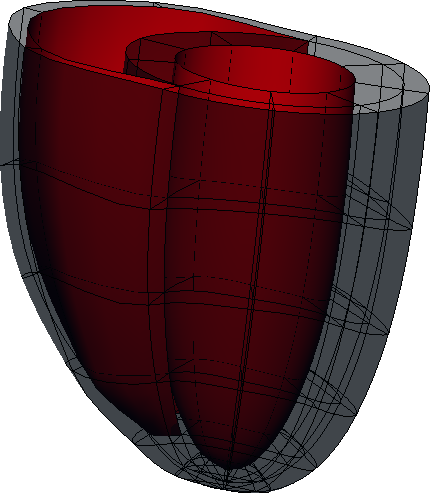
\includegraphics[width=.45\linewidth]{gfx/sham_mesh.png}}\quad
%     \subfloat[aortic-banded rat mesh.]
%     {\label{fig:ratrepmesh-b}
%     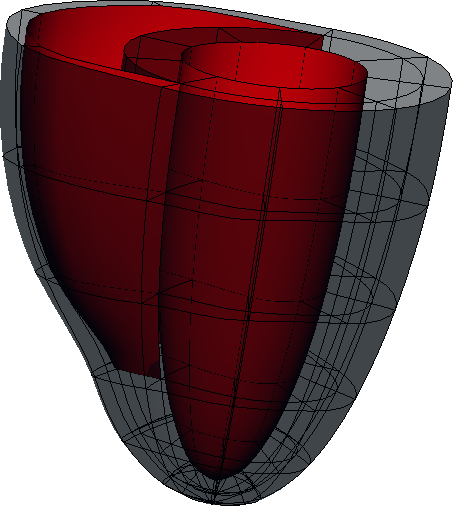
\includegraphics[width=.45\linewidth]{gfx/ab_mesh.png}}
%     \caption{Rat representative cubic Hermite finite element meshes.}\label{fig:ratrepmesh}
% \end{figure}

% \vspace{0.5cm}
% To mimic human pathological conditions, animal models are often established through life style, genetic or surgical procedures. In particular, left ventricular (LV) hypertrophy and compromised diastolic function can be caused by pressure overload, induced in rats by surgically constricting the aorta to impede blood flow. The constriction can be performed at different locations: transverse aorta, ascending aorta (shown in Figure~\ref{fig:aortic_banding}) or abdominal aorta, all causing an increase in aortic resistance and in LV end-diastolic pressure \cite{ku2016}. Cardiac hypertrophy and remodelling can be observed several weeks after the aortic constriction surgery. Since aortic constriction (especially in the abdominal aorta) requires simple experimental, surgical techniques \cite{ku2016}, aortic-banded (AB) rats are commonly used as an experimental animal model for HFpEF pathology \cite{patten2009, houser2012, conceicao2016, camacho2016}.

% % \begin{figure}[H]
% %     \centering
% %     \includegraphics[width=0.5\textwidth]{figures/aortic_banding_wiki.png}
% %     \caption{Aortic anatomy and one possible location for the banding (ascending aorta). Credit: Wikipedia.}
% %     \label{fig:aortic_banding}
% % \end{figure}

% \vspace{0.5cm}
% In the Introduction, we firstly introduce cardiac physiology. In that context, we will understand the importance of $\Ca$ ion, which represents the interface between the electrophysiological system and the mechanical system. We then provide a review of cardiac modelling, before summarising the work to date on simulating the rat heart.


